                         %%%   LOGIC   %%%
\chapter {Logic}
Logic is foundational for all of science and math. For computer science it is important to recall that most computers are logic machines. While logic can be studied using language, as was the liberal arts tradition, we abstract away the language and deal with a pure symbolic logic and that will be our focus. Since you are already well familar with how to construct Boolean expressions in some programming language we expect you will easily understand the development. Your instructor introduce the fascinating subject of natural language to the strict symbolic language forms in lecture and/or exercises. We will use this symbolic logic to prove things about any domain that can be represented using propositions and predicates.


\section {Propositional Logic}
\begin {definition}[Proposition] \index{proposition}
A proposition is a declarative sentence which is true or false, but not both. Also called a statement. In symbolic logic we use single lowercase letters beginning with p to represent propositions. These are called \textit{propositional variables}.
\end {definition}

\marginpar{A sentence with variables are not propositions. Pronouns function as variables since the antecedent of the pronoun is ambiguous.}

\begin{notes}
 There are two \textbf{literal values} in this logic, one that represents true and the other that represents false. Most commonly T is used for true and F for false. It is also common to use 1 for true and 0 for false. Many computer implementations do this, sometimes with unintended consequences. Questions (interogatives) and commands (statements in the imperative mood) are not propositions since no truth value can be associated with them. The \textbf{truth value} of a proposition is true, denoted by the logical literal T, if it is a true proposition, and the truth value of a proposition is false, denoted by F, it it is a false proposition. The area of logic that deals with propositions is called the \textbf{propositonal calculus} or \textbf{propositional logic}. 
\end{notes}

\subsection{Atomic and Compound Propositions and Logical Connectives}
\begin {definition}[Logical Connectives and Compound Propositions]\index{compound proposition}\index{logical connective}
A \textbf{compound proposition} is a proposition formed from atomic propositions with logical connectives or logical operators. Also called a logical or Boolean expression. An atomic propositions is one that is not a compound propositions.
\end {definition}

Note Schaum's represents an abstract compound proposition P with atomic propositions p,q,r, etc as P(p,q,r,...).

\begin {definition}[Negation]\index{negation}
Let $p$ be a proposition. The \textit{negation of p}, denoted by $\lnot p$ (also denoted by $\overline{p}$, is the statement 
\textit{"It is not the case that $p$."}\\
The proposition $\lnot p$ is read "not $p$". The truth value of the negation of $p$,  $\lnot p$, is the opposite of the truth value of $p$. Other notations for logical negation include $\neg$ and $\sim$. Many computer science students will use the ! symbol as well.
\end {definition} 

Note how you can always negate a natural language proposition by prepending the phrase, "it is not the case that..." followed by the original proposition.

\begin{definition}[Truth Table]\index{truth table}
Compound propositions are often presented in a table which shows the truth value associated with the expression for every possible combination of the atomic propositions in that compound proposition. The order of the rows most commonly starts with true for all atomic propositions and proceeds by alternating the rightmost atomic proposition between true and false with changes in the next leftmost proposition until all possible combinations have been listed. Table \ref{table:negation} displays the \textbf{truth table} for the negation of a proposition. The negation symbol is a unary operator taking as the single operand the proposition and giving a new propositon which is the negation of the given proposition. 
\end{definition}
    
   \begin{table}[htbp]
   \centering
   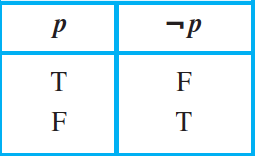
\includegraphics [width=1.5in]{Table-1-1-1-Negation}
   \caption{The Truth Table for the Negation of a Proposition}
   \label{table:negation}
   \end{table}

\begin {definition}[Conjunction]\index{conjunction}
 Let $p$ and $q$ be propositions. The \textit{conjunction} of $p$ and $q$, denoted by $ p \land q$, is the proposition \textit{p and q}. The conjunction $p \land q$ is true when both $p$ and $q$ are true and is false otherwise.
\end {definition}

\begin {definition}[Disjunction]\index{disjunction}
Let $p$ and $q$ be propositIons. The disjunction of $p$ and $q$, denoted by $p \lor q$, is the proposition \textit{p or q}. The disjunction $p \lor q$ is false when both $p$ and $q$ are false and true otherwise.
\end {definition}

Logical disjunction captures part of the meaning of the natural language word "or." But logical disjunction must be carefully observed to have a distinct formal meaning. Contrast this with what is called the exclusive or.

\begin {definition}[Exclusive OR]\index{exclusive OR}
Let p and q b propsition. The \textit{exclusive or} of $p$ and $q$, denoted by $p \oplus q$, is the proposition that is true when exactly one of $p$ and $q$ is true and is false otherwise.
\end {definition}

\subsection {Conditional Statements or Logical Implication}
\begin {definition}\index{implication}\index {antecedent}\index{conditional statement}\index{hypothesis}\index{premise}\index{conclusion}\index{consequent} 
Let $p$ and $q$ be propositions. The conditional statement $p \rightarrow $q is the proposition "if p then q".  The conditional statement $p \rightarrow q$ is false when $p$ is true and $q$ is false, and true otherwise. In the conditional statement  $p \rightarrow q$, $p$ is called the \textbf{hypothesis} (or \textbf{antecedent} or \textbf{premise})( and $q$ is called the \textbf{conclusion}, \textbf{consequent}. There are many ways in which the implication is set in type. Alternatives to what is defined here include  $\implies$ and $\supset$. It is acceptable to use -> when typing. 
\end {definition}

\begin{notes}
logical implication is not causality. When the antecedent is false the expression is always true. The only way the expression is false is when the antecedent is true and the consequence is false. \\

this is a logical operator and must not be confused with the use of the conditional statement in programmng languages. We will discuss this again in the section on Algorithms.

Conditional statements are a backbone of deductive logic and mathematical reasoning. Yet students often fail to grasp how to understand and use these statements. The lack of understanding here will hamper the ability to avoid many errors in understanding and writing mathematical proofs. 

The conditional statement is also called material implication. In a logic class you will also come across this concept as necessary and sufficient conditions. In logic, the necessary condition is the consequent of the conditional statement. We saw that a material implication is only false when the antecedent is true and the consequent is false. So if we find that the consequent is true and the implication is true, the antecedent MUST BE TRUE. 

Logic also teaches sufficient conditions. The sufficient condition is the antecedent. But having the antecedent be true and the implication be true does not guarantee us that the consequent will also be true. For example, "If you get an A on your final, then you will get an A for the course." Is it necessary for you to get an A on the midterm to get an A in the course? The material implication can still be true even when you got a B on the final, that is you get an A even though it is not the case that you got an A on the final. Getting an A on the final is sufficient for you to get an A in the course but it is not necessary for you to earn an A on the final to get an A for the course.

It will help you if you take the time to understand necessary and sufficient in the context of the material implication.
\end{notes}



\begin {definition} [Inverse, Converse and Contrapositive]\index{inverse}\index{converse}\index{contrapositive}
Given a conditional statement $p \rightarrow q$, its \textbf{inverse} is the statement $q \rightarrow p$, its converse is $\lnot p \rightarrow \lnot p$ and its \textbf{contrapositive} is the statement $\lnot q \rightarrow \lnot p $
\end {definition}
 
\begin {definition}[The Bi-Conditional]\index{bi-conditional}
Let $p$ and $q$ be propositions. The \textit{biconditional statement} $p \leftrightarrow q$ is the proposition "$p$ if and only if $q$." The biconditional statement $p \leftrightarrow q$ is true when $p$ and $q$ have the same truth values, an d is false otherwise. Biconditional statements are also called \textit{bi-implicatons}. We can also read this as "p is logically equivalent to q". 
 \end {definition}

 Note that you get the same truth values for the compound expressions $(p \leftrightarrow q)  \land (q \rightarrow p)$ and $p \leftrightarrow q$.
 
\begin{table}[htbp]
   \centering
   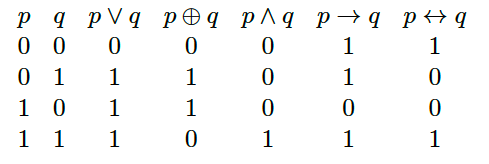
\includegraphics [width=3in]{Table-1-1-9-TableOfBitwiseLogic}
   \caption{Bitwise Logic}
   \label{table:bitwiselogic}
\end{table}

     \subsection{Evaluation of Compound Propositions}
Without parentheses compound logical statements can be ambiguous. But always explicitly including the parentheses leads to large numbers of them and makes the expressions harder to read. To avoid a large number of parentheses we adopt a convention of \textbf{operator precedence}. See Table \ref{table:precedenceOfLogicalOperators}.

\begin{table}[htbp]
   \centering
   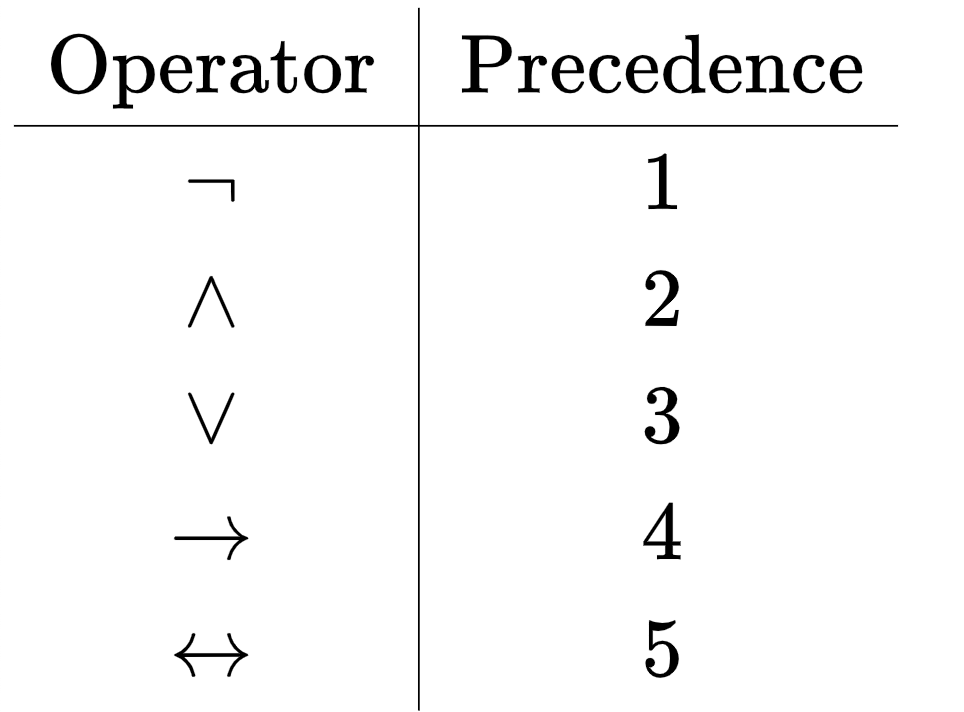
\includegraphics [width=1.5in]{PrecedenceOfLogicalOperators}
   \caption{Precedence of Logical Operators}
   \label{table:precedenceOfLogicalOperators}
\end{table}

      Truth Tables can be used to help derive the truth value of complex compound logic statements. Take the innermost binary operations required by the rules of precedence and create a column. Give the truth values for that small compound statement and then build up until you have the entire statement. 

    \subsection {Propositional Consistency}
consistent statements
    \subsection {Propositional Satisfiability}
\begin{definition}\index{satisfiability}
A compound proposition is \textbf{satisfiable} if there is an assignment of truth values to the variables in the compound proposition that makes the statement form true.
\end{definition}

\subsection{Paradox}
Some declarative statements defy a truth value. For example, ``This statement is false'' cannot be given a consistent truth value. If it is true, that the statement is false, then it must be true contradicting the assertion. Such a statement is called a \textbf{paradox}.


\begin {definition}\index{bit string}
A bit is a binary digit, typically a zero or a one. A bit string is a sequence of zero or more bits. The length of this string is the number of bits in the string. Given two bit strings of the same length we define bitwise operations:
\begin{enumerate}
\item bitwise OR, 
\item bitwise AND, 
\item bitwise XOR.
\end {enumerate}
\end{definition}





\subsection {Propositional Equivalences}

\begin {definition}[Tautology and Contradiction]\index{tautology}\index{contradiction}
A compound proposition that is always true , no matter what the truth value of the poisitons that occur in it, is called a \textit{tautology}. A compound proposition that is always false is called a \textit{contradiction}. A compound proposition that is neither a tautology nor a contradiction is called a \textit{contingency}.
\end {definition}

\begin {definition}[Logical Equivalence]\index{logical equivalence}
The compound proposition $p$ and $q$ are called \textit{logically equivalent} if $p \leftrightarrow q$ is  tautology. The notation $p \equiv q$ denotes that $p$ and $q$ are logically equivalent.
\end {definition}

Note: The symbol $\equiv$ is not a logical connective and $p \equiv q$ is not a compound proposition but a statement that $p \leftrightarrow q$ is a tautology. 

Two distinct propositions may evaluate to the same truth value for each combination of the atomic truth values. These two propositions are said to be logically equivalent or simply equivalent. This can be shown with a truth table and constitutes a valid proof of the equivalence. Logical equivalence leads to the principle that if two compound propositions always have the same truth values regardless of the values of the atomic propositions, then one can be substituted for the other where ever it appears.

  

  \begin{table}[htbp]
  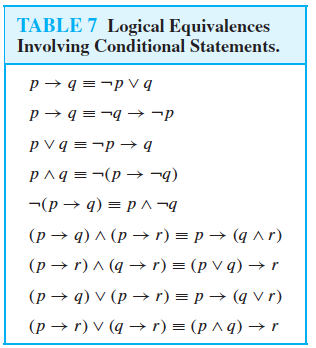
\includegraphics [width=3in]{Table-1-6-7-LogicalEquivalencesInvolvingConditionalStatements}
  \caption{Logical Equivalences Involving Conditional Statements}
  \label{table:logicalequivalencesinvolvingconditionalstatements}
  \end{table}
  
  \begin{table}[htbp]
  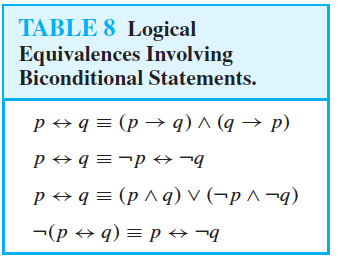
\includegraphics [width=3in]{Table-1-6-8-LogicalEquivalencesInvolvingBiconditonalStatements}
  \caption{Logical Equivalences Involving Bi-Conditional Statements}
  \label{table:LogicalEquivalenceInvolvingBiconditionalStatements}
  \end{table}

\begin{table}[htbp]
  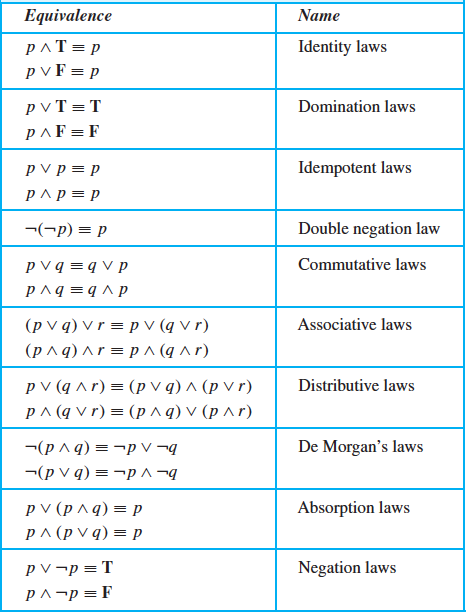
\includegraphics [width=3in]{Table-1-3-6-LogicalEquivalences}
  \caption{Logical Equivalences}
  \label{table:LogicalEquivalence}
  \end{table}




\section {Predicate Logic}
Predicate Logic. First order logic. There are other higher order logics. 
Propositional logic, zero order logic, cannot help with obviously true statements like, "Socrates is a man, all men are mortal, therefore Socrates is mortal". We need to introduce a way to prove such truths. This is called Predicate Logic or Predicate Calculus.

    \subsection {Predicates}
Some objects can have a property. A person may be tall or short. A number may be greater than 100. When we use variables to represent these objects we need a way to test them for the presence or absence of the quality we care about. We call these \textbf{propositional functions} and we call the quality being checked for \textbf{predicates}. 

For example, we may have a variable $x$ which is an integer. We can have a predicate which tests it to see if it is greater than 100. The predicate is "... is greater than 100" and we apply that to the variable $x$.

\begin{definition}[Predicate]\index{predicate}
A \textit{predicate} is a function which when applied to an object will evaluate to true when some property is present and false otherwise. We denote the predicate using a capital letter and write the expression using a functional notation. So the predicate $P$ when applied to the variable $x$ is written $P(x)$ and will take on the value of true or false when the value of $x$ has been fixed (bound).

Predicates are not limited to one argument but can have any number of arguments, called \textit{n-place predicates}. For example the predicate $S$ could be "...have the same color" and can accept pieces of fruit as objects. Then the expression $S(p,q,r,s,t)$ will be true if the color of each piece of fruit $p,q,r,s,t$ matches the others and false otherwise.

We often define a predicate using the notation, $P: x+1 > x$.
\end{definition}

\begin{notes}
More advanced texts may discard the parentheses around the arguments in a propositional function
\end{notes}

\begin{definition}{Value Assignment}
When we wish to indicate that a variable has been bound to a value, we use an assignment statement. We denote the assignment of the value c to the variable x with this notation: $x := c$. Some authors use $x\leftarrow c$ and many programming languages do this wil an equals sign, $x=c$. It helps to notice that there is an implied change of state from before and after the assignment. For example $t:=t+1$ must be understood to refer to the value of $t$ before the assignment while evaluating the expression and changing the value of $t$ with the assignment.
\end{definition}

We saw that the statement $x>2$ was not a proposition since $x$ is a variable. But once the variable is bound to a value it then has a truth value. We can denote this using this notation:
$[x:=1, (x>2)]$ and this will evaluate to false. We can also do this symbolically like this: $G:x>2$, [x:=3, G(x)] which will evaluate to true.

\subsection{Multi-place Predicates}
Some predicates take more than one variable. For example if we want to compare the color of two pieces of fruit, we can do it like so: $ASetOfFruit=\{apple, banana, papaya, grape,strawberry\}$, $SameColor(x,y):x is the same color as y$, $SameColor(apple,strawberry)=trie$, assuming the apple and the strawberry are both red.

Note how we specified that the variables are drawn from some set, which is called the \textbf{domain of discourse}. 

   \subsection {Quantifiers}\index{quantifier}\index{quantification}
Variables can be bound to values. But we often wish to assert a proposition over a range of values or to claim that there is an object with some property. This process of creating a proposition over some range of objects is called \textit{quantification}. The two fundamental quantifications are the universal and the existential.

        \subsubsection {Universal Quantification}\index{universe of discourse}\index{domain}
Many mathematical statements assert that a property is true for all values of a variable in a partiocular doman, called the \textbf{domain of discourse} (or \textbf{universe of discourse}, often just referred to s the \textbf{domain}. Such a statement is expressed using universal quantification. The universal quantification of $P(x)$ for a particular doman in the proposition that asserts that $P(x)$ is true for all values of $x$ in this domain. Note that the domain specifies the possible values of the variable $x$. The meaning of the universal quantification of $P(x)$ changes when we change the domain. The domain must always be specified when a universal quantifier is used; without it, the universal quantification of a statement is not defined.

\begin{definition}[Universal Quantification]\index{universal quantification}
The universal quantification of P(x) is the statement 
$$\text{"}P(x) \text{ for all values of }x \text{ in the domain."}$$
The notation $\forall x P(x)$ denotes the universal quantification of $P(x)$. Here $\forall$ is called the universal quantifier. We read $\forall x P(x)$ as "for all x P(x)" or "for every x P(x)". An element for which $P(x)$ is false is called a counterexample of $\forall x P(x)$.
\end{definition}

\begin{notes}
A domain of discourse must be provided when using universal instantiation. Generally an implicit assumption is made that all domains of discourse for quantifiers are nonempty. Note that if the domain is empty, then $\forall P(x)$ is true for any propositional function $P(X)$ because there are no elements $x$ in the domain for which $P(x)$ is false. 
\end{notes}

The changing the domain of discourse can change the evaluation of the predicate. For example if $P(x): x is purple$, if I wish to say that all eggplants are purple, I can say that when talking about eggplants, $\forall x P(x)$ is true but when talking about apples it is not true that $\forall x P(x)$. If you were to show me an eggplant that is not purple, you have given me a \textbf{counter example} and that will refute my assertion that all eggplants are purple. A single counter example is sufficient to refute a universal claim.

In the domain of natural numbers, what is the truth value of this assertion? $\forall n: n+1 > n$?

Consider $R:x^2 \ge x$ and the assertion $\forall x: R(x)$ in the domain of integers. Now consider it for the domain of reals.

It is sometimes helpful to think of a universal quantification as the conjunction of all elements in the domain when the domain is finite. For example if n is a natural number, $\forall n P(n) \equiv P(0) \land P(1) \land \dots \land P(n)$.

Translation challenge: All apples are sweet. $A(x): x is an apple$, $S(x): x is sweet$. Do you translate as $\forall x A(x) \land S(x)$ if the domain of discourse is the set of all fruits? No. It must be $\forall x A(x) \rightarrow S(x)$. Otherwise you are saying all fruits are sweet apples. 


        \subsection {Existential Quantifier}
Many mathematical statements assert that there is an element with a certain property. For example, for any integer $i$ there is another integer $j$ such that $i+j=0$. Such statements are expressed using existential quantification. With existential quantification, we for a proposition that is true if and only if $P(x)$ is true for at least one value of $x$ in the domain.

\begin{definition}\index{existential quantification}\index{existential quantifier}
The \textit{existential quantification} of $P(x)$ is the proposition
$$\text{"There exists an element }x \text{ in the domain such that } P(x) \text{ ."}$$
We use the notation $\exists x P(x)$ for the existential quantification of $P(x)$. Here $\exists$ is called the \textbf{existential quantifier}.
The domain must always be specified when a statement $\exists P(x)$ is used. The meaning of $\exists P(x)$ changes when the domain changes. without specifying the domain, the statement $\exists P(x)$ has no meaning. The existential quantifier $\exists P(x)$ is read as, "There is an $x$ such that $P(x)$, "There is at least one $x$ such that $P(x)$", or "For some $x P(x)$".
\end{definition}

\begin{notes}
Generally, an implicit assumption is made that all domains of discourse for quantifiers are nonempty. If the domain is empty, the $\exists P(x)$ is false whenever $P(X)$ is a propositional function because when the domain is empty, there can be no element in the domain for which $P(x)$ is true.\\

For finite domains, the existential quantifier can be thought of as a disjunction. For $n$ a natural number, $\exists n P(n)$ can be rewritten as $P(0) \lor P(1) \lor \dots \lor P(n)$.
\end{notes}

    \subsection {Other Quantifiers}
You will sometimes see other quantifiers but the only one which occurs often enough to get notice is the uniqueness quantifier:

\begin{definition}
The \textit{uniqueness quantification} of $P(x)$ is the proposition:
$$\text{"There exists exactly one element }x \text{ in the domain such that }P(x)\text{".}$$
We use the notation $\exists !$ for the uniqueness quantification.
\end{definition}

    \subsection {Quantifiers with Restricted Domains}
An abbreviated notation is sometimes used to specify some subset of the domain. For example $\forall x <0 (x^2 >0)$ in the domain of real numbers places the restrictive clause next to the quantifier.

The truth of an existential statement is proven by demonstrating one object that makes the predicate true. We call that object the \textit{witness}. To show that an existential statement is false we must show that no such object from the domain will make the predicate true. We must prove a negative. For example, if I assert that in the reals, $\exists x: x=x+1$, you cannot produce any such $x$. You could argue that the predicate is a contradiction since the equation $x=x+1$ is equivalent to $1=0$ which is clearly a contradiction. But many existential statements are not that easily proven false.

  

    
\begin{definition}[Binding Variables]\index{binding}
When a variable has been assigned a value, we say the value has been \textbf{bound} to the variable. Any variable that has not yet been bound to a value is said to be \textbf{free}. The \textbf{scope} of the binding is controlled by the use of parentheses or other marks. The value of a variable is also bound by the use of a quantifier and the variable is either within or outside the scope of that quantifier.
\end{definition}

Care must be taken  with quantified statements regarding the scope of the binding. When a variable is bound to a quantifier, all instances of that variable within the scope are bound. Any use of that variable outside the scope is unbound, or free. Within the scope of the binding a variable can be changed with no effect on the logic. For example $\forall a (Q(a) \land P(a))$, the quantifier binds $a$. We can rewrite this as $\forall b(Q(b) \land P(b))$. But if the expression is $\forall a Q(a) \land P(a)$, the first predicate is bound to the universal quantification but the second is not. The second use is \textit{unbound} or \textit{free}. Another example would be $\exists x:(x+y>x)$ the variable $x$ is bound but the variable $y$ is free.

\subsection {Precedence of Quantifiers}
We must update the precedence of the operators. Parentheses are still the  highest. But quantifiers come before propositional operators. The order of precedence places all propositional operators ahead of quantifiers. All quantifiers are equal precendence.


    \subsection {Logical Equivalences Involving Quantifiers}
\begin{definition}
Statements involving predicates and quantifier are \textit{logically equivalent} if and only if they have trhe same truth value no matter which predicates are substitued into these staeent and which domain of discourse is used for the variables in these propositionan functions. We use the notation $S \equiv T$ to indicate that two statements $S$ and $T$ involving predicates and quantifiers are logically equivalent.
\end{definition}

$\forall x (P(x) \land Q(x)) \equiv \forall x P(x) \land \forall x Q(x)$ regardless of the domain. 

    \subsection {Negating Quantified Expressions}
$\neg \forall x P(x) \equiv \exists x \neg P(x)$ is a logical equivalence.
$\neg \exists x P(x) \equiv \forall x \neg P(x)$ is a logical equivalence.
These are DeMorgan's laws again, this time for quantified statements. 
    
    \begin{table}[htbp]
  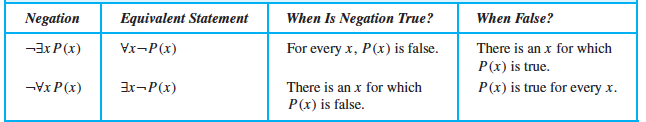
\includegraphics [width=3in]{DeMorgansForQuantifiedExpressions}
  \caption{DeMorgansForQuantifiedExpressions}
  \label{table:DeMorgansForQuantifiedExpressions}
  \end{table}
      
 


   \subsection {Nested Quantifiers and their Order}
   \begin{table}[htbp]
   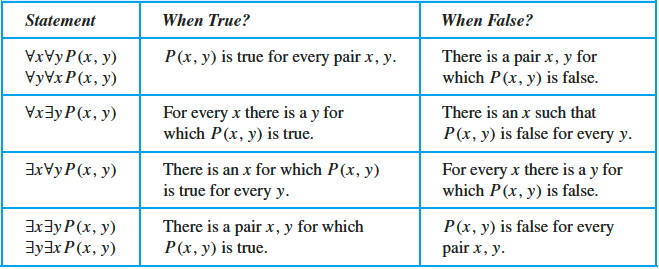
\includegraphics [width=3in]{Table-1-4-1-QuantificationOfTwoVariables}
  \caption{Quantification Of Two Variables}
  \label{table:QuantificationOfTwoVariables}
  \end{table}
  
It is important to note that the order of the quantifiers can make a difference. For example is this statement true or false for the domain of integers? $\forall x \exists y : (x+y=10)$. This is easily proven true with a bit of algebra. But what about $\exists y \forall x : (x+y=100)$. This is false since there is no such integer that will always give 10 when added to any other integer. 
 
  Universal quantifiers at the outermost level can be omitted, i.e., free variables are interpreted as universally quantified at the outermost level. Quantifiers can be applied to more than one variable at once (e.g., forall x,y). The infix equality sign (e.g., x = y) can be used as a shorthand for the equality predicate (e.g., equals(x,y)).
   \newpage 
    \subsection {Negating Nested Quantifiers}

Table-1-5-1-QuantificationsOfTwoVariables
\begin{table}[htbp]
  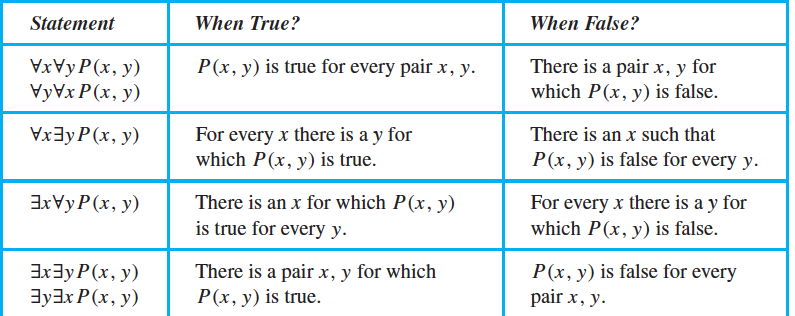
\includegraphics [width=3in]{Table-1-5-1-QuantificationsOfTwoVariables}
  \caption{Quant Of 2 Var}
  \label{table:QuantificationOfTwoVariables}
  \end{table}
  
\subsection{Thinking of Quantification as Loops}

THINKING OF QUANTIFICATION AS LOOPS In working with quantifications of more
than one variable, it is sometimes helpful to think in terms of nested loops. (Of course, if there
are infinitely many elements in the domain of some variable, we cannot actually loop through
all values. Nevertheless, this way of thinking is helpful in understanding nested quantifiers.) For
example, to see whether $\forall x \forall yP(x, y)$ is true, we loop through the values for $x$, and for each $x$
we loop through the values for $y$. If we find that $P(x, y)$ is true for all values for $x$ and $y$, we
have determined that $\forall x\forall yP(x, y)$ is true. If we ever hit a value $x$ for which we hit a value $y$
for which $P(x, y)$ is false, we have shown that $\forall x\forall yP(x, y)$ is false.
Similarly, to determine whether $\forall x\exists yP(x, y)$ is true, we loop through the values for $x$.
For each $x$ we loop through the values for $y$ until we find a $y$ for which $P(x, y)$ is true. If for
every $x$ we hit such a $y$, then $\forall x \exists yP(x, y)$ is true; if for some $x$ we never hit such a $y$, then
$\forall x\exists y P(x, y)$ is false.

To see whether $\exists x\forall yP(x, y)$ is true, we loop through the values for $x$ until we find an $x$ for
which $P(x, y)$ is always true when we loop through all values for $y$. Once we find such an $x$, we
knowthat $\exists x\forall yP(x, y)$ is true. If we never hit such an $x$, then we know that $\exists x\forall yP(x, y)$ is false.

Finally, to see whether $\exists x\exists yP(x, y)$ is true, we loop through the values for $x$, where for
each $x$ we loop through the values for $y$ until we hit an $x$ for which we hit a $y$ for which $P(x, y)$
is true. The statement $\exists x\exists yP(x, y)$ is false only if we never hit an $x$ for which we hit a $y$ such that $P(x, y)$ is true.

$S(x): x is a man$, $M(x): x is mortal$. Express ``all men are mortal, Socrates is a man, therefore Socrates is mortal''. $S(Socrates) \forall x S(x) \rightarrow M(x)$  (move to proofs where inference rule is discussed.)


   \subsection {Logic Programming}
An important type of programming language is designed to reason using the rules of predicate
logic. Prolog (from Programming in Logic), developed in the 1970s by computer scientists
working in the area of artificial intelligence, is an example of such a language. Prolog programs
include a set of declarations consisting of two types of statements, Prolog facts and Prolog
rules. Prolog facts define predicates by specifying the elements that satisfy these predicates.
Prolog rules are used to define new predicates using those already defined by Prolog facts.

